%%
%% Copyright 2007-2020 Elsevier Ltd
%%
%% This file is part of the 'Elsarticle Bundle'.
%% ---------------------------------------------
%%
%% It may be distributed under the conditions of the LaTeX Project Public
%% License, either version 1.2 of this license or (at your option) any
%% later version.  The latest version of this license is in
%%    http://www.latex-project.org/lppl.txt
%% and version 1.2 or later is part of all distributions of LaTeX
%% version 1999/12/01 or later.
%%
%% The list of all files belonging to the 'Elsarticle Bundle' is
%% given in the file `manifest.txt'.
%%

%% Template article for Elsevier's document class `elsarticle'
%% with numbered style bibliographic references
%% SP 2008/03/01
%%
%%
%%
%% $Id: elsarticle-template-num.tex 190 2020-11-23 11:12:32Z rishi $
%%
%%
\documentclass[preprint,12pt]{elsarticle}

%% Use the option review to obtain double line spacing
%% \documentclass[authoryear,preprint,review,12pt]{elsarticle}

%% Use the options 1p,twocolumn; 3p; 3p,twocolumn; 5p; or 5p,twocolumn
%% for a journal layout:
%% \documentclass[final,1p,times]{elsarticle}
%% \documentclass[final,1p,times,twocolumn]{elsarticle}
%% \documentclass[final,3p,times]{elsarticle}
%% \documentclass[final,3p,times,twocolumn]{elsarticle}
%% \documentclass[final,5p,times]{elsarticle}
%% \documentclass[final,5p,times,twocolumn]{elsarticle}

%% For including figures, graphicx.sty has been loaded in
%% elsarticle.cls. If you prefer to use the old commands
%% please give \usepackage{epsfig}

%% The amssymb package provides various useful mathematical symbols
\usepackage{amssymb}
%% The amsthm package provides extended theorem environments
%% \usepackage{amsthm}
\usepackage{graphicx}
%\usepackage{caption}
\usepackage{comment}
\usepackage{amsmath}
\usepackage{subfigure}
\usepackage{booktabs}
\usepackage{float}
%\usepackage{pgfplots}
\usepackage{graphicx}
\usepackage{fullpage} % for full page width
\usepackage{lipsum} % for dummy text
\usepackage{adjustbox} % for adjusting graphics

\usepackage{hyperref}
\hypersetup{
     colorlinks=true,
     linkcolor=black,
     citecolor=black,
     filecolor=black,
     urlcolor=black,
 }

%% The lineno packages adds line numbers. Start line numbering with
%% \begin{linenumbers}, end it with \end{linenumbers}. Or switch it on
%% for the whole article with \linenumbers.
%% \usepackage{lineno}

\journal{Computer Methods in Applied Mechanics and Engineering}

\begin{document}

\begin{frontmatter}

%% Title, authors and addresses

%% use the tnoteref command within \title for footnotes;
%% use the tnotetext command for theassociated footnote;
%% use the fnref command within \author or \address for footnotes;
%% use the fntext command for theassociated footnote;
%% use the corref command within \author for corresponding author footnotes;
%% use the cortext command for theassociated footnote;
%% use the ead command for the email address,
%% and the form \ead[url] for the home page:
%% \title{Title\tnoteref{label1}}
%% \tnotetext[label1]{}
%% \author{Name\corref{cor1}\fnref{label2}}
%% \ead{email address}
%% \ead[url]{home page}
%% \fntext[label2]{}
%% \cortext[cor1]{}
%% \affiliation{organization={},
%%             addressline={},
%%             city={},
%%             postcode={},
%%             state={},
%%             country={}}
%% \fntext[label3]{}

\title{Enhancing Fractographic Fatigue Failure Analysis, Automated Flow Stress, and Fracture Toughness Evaluation in Fatigue Specimens - a Smart Approach with Artificial Intelligence and Image Processing}

%% use optional labels to link authors explicitly to addresses:
%% \author[label1,label2]{}
%% \affiliation[label1]{organization={},
%%             addressline={},
%%             city={},
%%             postcode={},
%%             state={},
%%             country={}}
%%
%% \affiliation[label2]{organization={},
%%             addressline={},
%%             city={},
%%             postcode={},
%%             state={},
%%             country={}}
\author[Computer_a]{Avichay Mazin}
\author[Computer_a]{Jonatan Boritski}
\author[Computer_b]{Or Anijar}
\author[Computer_a]{Sapir Dahan}
\author[soreq]{Elad Farkash}
\author[fracture]{Mor Mega}
%\author[Computer_a,Computer_a,Computer_b]{Avichay Mazin$^a$, Jonatan Boritski$^a$, Or Anijar$^b$, Sapir Dahan$^a$, Elad Farkash$^c$, Mor Mega$^d$}

\affiliation[Computer_a]{organization={Department of Computer Science, \\Ariel University},%Department and Organization
            city={Ariel},
            postcode={40700},
            country={Israel}}

\affiliation[Computer_b]{organization={Department of Computer Science, \\Ariel University},%Department and Organization
            city={Ariel},
            postcode={40700},
            country={Israel}}

\affiliation[soreq]{organization={Soreq Nuclear Research Center},%Department and Organization
            city={Yavne},
            postcode={81800},
            country={Israel}}

\affiliation[fracture]{organization={The Fracture and Fatigue Research Laboratory, \\Department of Mechanical Engineering and Mechatronics, \\Ariel University},%Department and Organization
            city={Ariel},
            postcode={40700},
            country={Israel}}

\begin{abstract}
%% Text of abstract

\end{abstract}

%%Graphical abstract
\begin{graphicalabstract}
%\includegraphics{grabs}
\end{graphicalabstract}

%%Research highlights
\begin{highlights}
\item Research highlight 1
\item Research highlight 2
\end{highlights}

\begin{keyword}
%% keywords here, in the form: keyword \sep keyword

%% PACS codes here, in the form: \PACS code \sep code

%% MSC codes here, in the form: \MSC code \sep code
%% or \MSC[2008] code \sep code (2000 is the default)

\end{keyword}

\end{frontmatter}

%% \linenumbers

%% main text
\section{Introduction}
\label{Sec:Introduction}

\begin{comment}
\subsection{Today Scene: What We Have and What Might Evolve}  \label{Subsec:Today's Scene: What We Have and What Might Evolve}
The application of machine learning and deep learning for analyzing fracture surfaces and extracting meaningful information has seen a significant rise in the last years as discussed in a study \cite{tsopanidis2020unsupervised}.
As we can see in the article, these tools are not only facilitate the extraction of valuable insights that may surpass the capabilities of traditional fractographic experts, but also introduce automation, making the entire process more efficient and time saving.

In practical terms, utilizing machine and deep learning for fracture surface analysis proves to be a time saving effort. Instead of the manual analysis of fracture surfaces, which can be time consuming, these advanced tools simplify the process. Moreover, the accuracy and effectiveness of the analyses are often hig enough that, in certain cases, reliance on traditional fractographic experts may become unnecessary. The automated nature of machine and deep learning analyses contributes to a more efficient, rapid, and sometimes even superior understanding of fracture surfaces.
\par
As we explain earlier, an analysis of fatigue failure in engineering structures has already been done before in some aspects.
For example, in previous studies, some researchers have already made an analysis about fractions materials produced through 3D printing. One is the research \cite{anidjar2023transfer}.
 This research emphasize why is important to analyze fractures in materials and explain that fractographic analysis plays a crucial role in understanding the mechanical properties and fatigue behavior of materials, especially in identifying the primary causes of failure. For this problem, the challenge of identifying fatigue crack initiation sites, the researchers attitude towards the solution for the problem was innovation and efficiency. They recognized that the process of identifying and characterizing fatigue crack initiation sites in materials can be time consuming and costly when done manually. Therefore, they try to develop a computer vision based approach that could automate and expedite the process.
the researchers have been used in two deep learning algorithms. One is called ResNet152 and it used to filter out image sections that do not contain the fatigue crack initiation site. The second is called YOLOv5 which used for object detection. After the irrelevant image sections have been filtered out by ResNet152, YOLOv5 is trained to detect and classify the remaining image sections to precisely identify the initiation site.
\end{comment}


%\subsection{Mechanical Background}
Additive Manufacturing (AM) technology, also known as 3D printing, is an innovative process wherein parts are fabricated layer by layer, adhering to three-dimensional digital models. This innovative technique, emerged in the late 1980s, has made a significant advancement in manufacturing technology. Widely referred as a cornerstone of the third industrial revolution, AM offers almost unlimited opportunities for the creation of intricately designed products, which is markedly different from traditional metal manufacturing methods~\cite{wong2012review}. One of the big advantage of AM lies in its obviation of the need for molds, a factor that substantially diminishes production costs and enable producing of complex components~\cite{herzog2016additive}.


Titanium alloys are highly advanced structural materials known for their diverse set of exceptional properties. These include resistance to corrosion in seawater, impressive strength-to-weight ratios, excellent fracture toughness, high fatigue resistance, strong compatibility with composites, long-term durability with minimal maintenance requirements, and exceptional biocompatibility~\cite{qian2016additive}. Despite the extensive exploration of the static mechanical properties of AM materials, encompassing factors such as strength, stiffness, and impact energy~\cite{debroy2018additive,gorsse2017additive}, investigations into their dynamic performance and fatigue characteristics remain comparatively scant. Additive Ti-6Al-4V is increasingly esteemed as promising lightweight structural components in aerospace and automotive sectors~\cite{boyer1996overview,debroy2018additive}. In these areas, the ability to withstand fatigue loads is critical. However, a comprehensive understanding of its fatigue behavior and underlying failure mechanisms remains elusive. Hence, delving into the mechanical fatigue properties of AM materials becomes imperative.

Fatigue failure of engineering components and structures results from progressive fracture caused by cyclic or fluctuating loads. Fatigue is an important potential cause of mechanical failure because most engineering components or structures can be subjected to cyclic loads during their lifetime.
An abbreviated summary of fatigue processes and mechanisms: fatigue crack initiation, propagation, and final fracture. Characteristic fatigue fracture features that can be visually discerned under low magnification are then described.
Typical microscopic features observed on structural metals are presented.
\begin{comment}
    In \textcolor{red}{need more up to date papers if these are examples for papers that made use of the method we are using... If not, then examples of what are these?}~\cite{astiz1986incompatible,carpinteri1992stress,carpinteri1992elliptical}, models for predicting the stress intensity factor for such a geometry were proposed.
\end{comment}
\textcolor{green}{Additive Manufacturing\\Fatigue\\Fractografic analysis and surface regions\\stress intensity factor calculation models\\flow stress calculation models\\It may be useful to solve this using computer vision methods  (no equations, just references)}




%\subsection{Related Work}  \label{Subsec:Related Work}
    The integration of computer vision in the field of fracture mechanics, particularly in the analysis of metal fractures, has evolved significantly over recent years.
    In its early stages, the approach primarily relied on scanning Scanning Electron Microscope (SEM) images and conducting manual classification efforts.
    However, the traditional process is manual, labor-intensive, and prone to human error.
    Automating this process and developing quantitative methods for studying fracture surfaces is a major challenge but has significant industrial and scientific potential.
    Automated fractography could enhance the reliability of failure analysis and uncover new insights into material failure mechanisms.

    Early applications in fracture mechanics prioritized image processing over the more advanced computer vision and machine learning techniques.
    These initial approaches were designed to enhance features in images of fracture surfaces captured by SEM and optical microscopy, with a greater emphasis on qualitative rather than quantitative analysis.
    Fundamental techniques employed in these efforts included spatial domain methods like texture analysis and the Gray Level Co-occurrence Matrix (GLCM) for fractal analysis.
    \textcolor{red}{In \cite{zain2009enhancement}}, the authors experimented with various spatial filtering techniques such as mean, median, Gaussian, and Wiener filters to enhance the quality of identification of the fracture image.
    In the engineering field, another set of experiments can be observed \textcolor{red}{In \cite{das2011characterization}}, where the changes on the surface are effectively characterized using these methods.
    Furthermore, some of these techniques also incorporated transform domain methods, such as Fourier transform, wavelet transform, and Gabor transform.
    In another study, \textcolor{red}{In \cite{hu2017automation}}, the authors employed edge detection and peak-finding algorithms to determine the progression marks associated with fatigue crack growth.

    These methods were applied to optical and Scanning Electron Microscopy (SEM) images to classify and characterize fracture surfaces.
    However, these methods often required additional user input and assumptions, which limited their robustness and applicability, especially for complex surfaces.

    Recent developments have seen the use of machine learning and artificial intelligence in materials characterization, including micro-structure classification and defect analysis.
    Promising machine learning methods like artificial neural networks and support vector machines have played a pivotal role in classifying observed fractures, yielding promising results in materials characterization.
    Some notable achievements in this area include the use of a complex CNN architecture known as Unet,
    as demonstrated \textcolor{red}{In \cite{tsopanidis2020toward}}, where an accuracy of 71.2 percent in Intersection over Union (IOU) was achieved for triple-class classification,
    distinguishing inter-granular and trans-granular fracture events from scanning electron microscope images.
    Another article compared a more intricate Unet neural network architecture, reaching an accuracy of 0.86 percent in the Dice score accuracy metric for the segmentation task of detecting dimple fractures.

    A prominent trend has emerged in recent times where a fusion of traditional image processing methods and cutting-edge AI techniques has been observed.
    In these approaches, a pivotal role is played by feature extraction during the prepossessing phase, enhancing the salient characteristics within images.
    As exemplified \textcolor{red}{In \cite{naik2019identification}}, researchers combined texture recognition algorithms, specifically the Local Binary Pattern (LBP), with the classical machine algorithm called Linear Discriminant Analysis (LDA). This innovative combination allowed them to identify the fracture type and its area in both brittle and ductile materials by leveraging the uniqueness of texture features, achieving an impressive accuracy rate of 94 percent.
    Another notable example is presented \textcolor{red}{In \cite{bastidas2016fractographic}}, where SVM classification was employed.

    A groundbreaking advancement in this research lies in the integration of the localization problem with the feature extraction phase.
    As demonstrated \textcolor{red}{In \cite{zhang2023automated}}, a remarkable achievement was reached with a detection rate of up to 92 percent in terms of the F1 score for detecting bridge cracks.
    This approach was developed by segmenting the process into three distinct phases: initially selecting specific regions, then extracting features using methods like SIFT and HOG, and finally applying the YOLO neural network architecture for precise object localization and detection.


\textcolor{green}{In this study,...}






\section{Mechanical basic terms}  \label{sec:Basic terms}


Two failure criteria may be used to predict the final failure of a specimen subjected to cyclic fatigue loading. The first criterion is related to the flow stress parameter \(\sigma_{net}\), and the second is related to the stress intensity factor \(K_{I}\). Once one of these parameters reaches a critical value, failure is expected. The model used here to determine the flow stress in a bar specimen tested in cyclic fatigue is presented in Section~\ref{Subsec: Flow stress calculation model}.
In Section~\ref{Subsec: Stress intensity factors calculation model}, several closed-form solutions for the determination of \(K_I\) are introduced and the best one is chosen \cite{shin2004experimental}.


\subsection{Fractographic image analysis description}
\label{Subsec: Fractographic image analysis}

\subsection{Flow stress calculation model}
\label{Subsec: Flow stress calculation model}
\begin{figure*}[t!]
  \begin{center}
  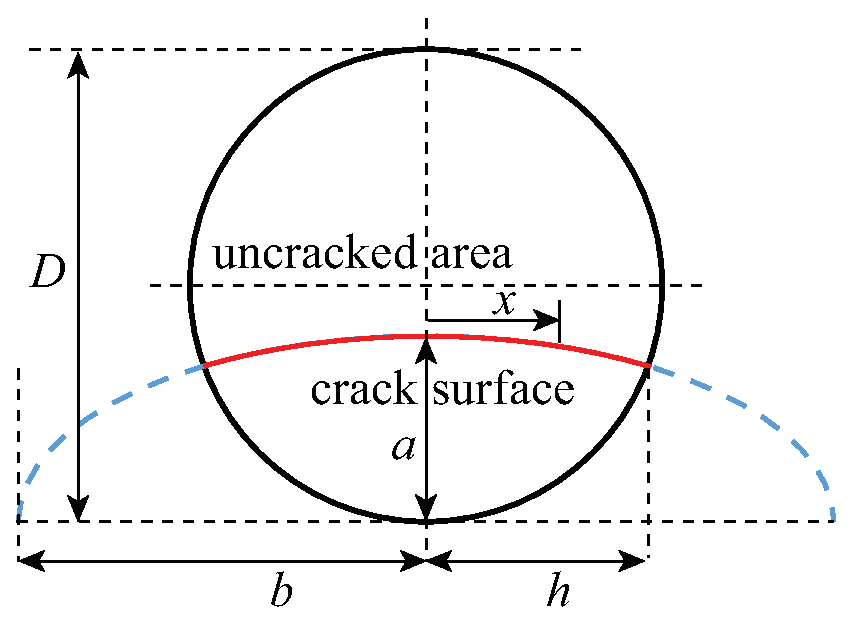
\includegraphics[width=3in]{elliptical_surface_crack.eps}
  \caption{Schematic view of an elliptical crack.}
  \label{fig:elliptical_crack}
   \end{center}
\end{figure*}

One known failure criterion is based on the calculated flow stress $\sigma_{net}$. Once this parameter reaches the failure stress $\sigma_{f}$, the final failure will occur.

The failure stress \(\sigma_{f}\) is related to the ligament area, defined as the uncracked area illustrated in Fig.~\ref{fig:elliptical_crack}. For a specific material, the value of \(\sigma_{f}\) is given by \cite{kanchanomai2004low}
%
\begin{equation}
    \sigma_{f} = \frac{\sigma_Y + \sigma_{UTS}}{2}
\end{equation}
%
where \(\sigma_Y\) is the yield stress and \(\sigma_{UTS}\) is the ultimate stress of the material.

The flow stress, \(\sigma_{net}\), is a function of the applied force and the uncracked area, namely,
%
\begin{equation}
\label{eq:sig_net}
\sigma_{net}= \displaystyle\frac{\sigma_{max} A_0}{A_{\textit{uncracked area}}}
\end{equation}
%
where $\sigma_{max}$ is the maximum applied stress in each fatigue cycle, \(A_0\) is the total area of the specimen surface, and \(A_{\text{uncracked area}}\) is the ligament area illustrated in Fig.~\ref{fig:elliptical_crack}. Once \(\sigma_{net}\) reaches the value of \(\sigma_f\), the specimen will fail.
%
%

\subsection{Stress intensity factor calculation model}
\label{Subsec: Stress intensity factors calculation model}
\textcolor{green}{add ellipse restrictions}
%
%
\begin{table}[t!]
\caption{Tabulated values of $M_{i,j,k}$ in eq.~(\ref{eq:F_I}). \strut}
\label{tab:M_ijk}      % Give a unique label
\resizebox{\columnwidth}{!}{
\begin{tabular}{cccclccclccc}
\noalign{\bigskip}\hline\noalign{\smallskip}\hline
  &          & k=0       &           &  &          & k=1       &          &  &         & k=2      &           \\ \cline{2-4} \cline{6-8} \cline{10-12}
j & i=0      & 1         & 2         &  & i=0      & 1         & 2        &  & i=0     & 1        & 2         \\
0 & 1.095    & -1.177    & 0.725     &  & 0.113    & 0.271     & -0.388   &  & -0.896  & 0.904    & 0.008     \\
1 & -1.336   & 17.924    & -17.427   &  & 1.824    & -11.649   & 10.074   &  & 3.092   & 0.701    & -4.883    \\
2 & 13.108   & -137.252  & 134.652   &  & -21.709  & 98.358    & -80.088  &  & -4.197  & -32.641  & 55.092    \\
3 & -43.689  & 545.816   & -551.902  &  & 105.483  & -415.027  & 328.165  &  & -13.255 & 204.104  & -305.079  \\
4 & 134.868  & -1223.334 & 1239.493  &  & -271.225 & 982.713   & -772.921 &  & 51.548  & -568.407 & 916.962   \\
5 & -242.653 & 1541.587  & -1548.537 &  & 387.47   & -1329.634 & 1055.952 &  & -59.329 & 857.543  & -1545.428 \\
6 & 254.093  & -1006.656 & 969.388   &  & -290.024 & 961.893   & -784.581 &  & 13.481  & -657.659 & 1372.595  \\
7 & -108.196 & 264.206   & -227.132  &  & 88.387   & -288.565  & 245.798  &  & 10.854  & 191.57   & -485.556  \\
\hline\noalign{\smallskip}\hline
\end{tabular}
}
\end{table}
An additional known failure criterion is based on the stress intensity factor $K_I$ value. Once this parameter reaches the fracture toughness $K_{Ic}$ of the tested material, the crack will propagate, and final failure will occur. The critical stress intensity factor or fracture toughness value \(K_{Ic}\) is reached once the crack approaches a critical size.



In~\cite{toribio2009automated}, it was demonstrated that the crack front in a fatigue bar specimen may be treated as an ellipse with the center located at the specimen surface, as illustrated in Fig.~\ref{fig:elliptical_crack}. The parameters $a$ and $b$ are the major and minor diameters of the ellipse in Fig.~\ref{fig:elliptical_crack}, respectively. These dimensions represent the depth and width of the crack, respectively. The parameter $D$ is the total specimen diameter, $x$ is a chosen coordinate between 0 and $h$ where $h$ is the horizontal distance between the center of the ellipse and the intersection between the ellipse and the specimen outer surface. It may be noted that the axis of symmetry of the ellipse is the same as the axis of symmetry of the bar and the center of the ellipse is on the edge of the rod. All parameters are shown in Fig.~\ref{fig:elliptical_crack} and may be used to calculate $K_I$.

Next, several closed-form solution are presented and the best one is chosen. In~\cite{valiente1980criterios}, the first closed-form solution was introduced. This form was only for a straight front crack ($b$ limit to infinity). The value of $K_I$ is calculated only at the center of the crack front.
In~\cite{astiz1986incompatible}, a closed-form solution is introduced for an elliptical crack front; but $K_I$ is found only in the center of the crack front. In~\cite{couroneau1998simplified,carpinteri1992elliptical} two closed-form solution were presented, one at the crack front center, shown as point A in Fig.~\ref{fig:elliptical_crack}, and another for the end of the crack front, shown as point G in Fig.~\ref{fig:elliptical_crack}. In \cite{shin2004experimental} a closed-form solution was found based on the FE method and the virtual crack extension technique~\cite{hellen1975method}. The solution was found as a function of $a$, $b$ and $x/h$ the location along the crack front, as shown in Fig.~\ref{fig:elliptical_crack}.
Another solution that use these three parameters~\cite{shih2002stress} was found to produce negative results. A detailed review on these solutions and other solutions may be found in~\cite{toribio2009automated}.
It was found~\cite{toribio2009automated} that the best closed-form solution for the problem in this research is~\cite{shih2002stress}.



\begin{comment}
The three dimensionless parameters used are the crack depth $H$, the ellipse ratio $r$, and the location along the crack front $X$. These parameters may be calculated as
\begin{equation}\label{eq:crack depth}
    H=\frac{D}{a}\;\;\;;\;\;\; r=\frac{a}{b} \;\;\;;\;\;\;X=\frac{x}{h}
\end{equation}
where $D$ and $a$ are the specimen diameter and the largest distance between the specimen surface and the ellipse along the specimen diameter, $a$ and $b$ are the major and minor diameters of the ellipse, $x$ is a chosen parameter between 0 and $h$ and $h$ is the horizontal distance between the center of the ellipse and the intersection between the ellipse and the specimen outer surface. All illustrated are illustrated in Fig.~(\ref{}).
\end{comment}



In~\cite{shin2004experimental}, the closed-form solution is based on the FE method and the virtual crack extension technique~\cite{hellen1975method}.  The calculation of \(K_I\) is proposed as
%
\begin{equation}
\label{eq:K_I__F_I}
K_{I}=F_I \sigma_0 \sqrt{\pi a}
\end{equation}
%
where $F_I$ is a function of $a, b, D, h$ and $x$ given as
%
\begin{equation}
\label{eq:F_I}
F_{I}=\sum^{2}_{i=0} \sum^{7}_{j=0}\sum^{2}_{k=0} M_{ijk}\left(\frac{a}{b}\right)^i  \left(\frac{a}{D}\right)^j  \left(\frac{x}{h}\right)^k\;\;.
\end{equation}
In eq.~(\ref{eq:F_I}) the coefficients $M_{ijk}$ were determined from FEAs in \cite{shin2004experimental} and presented in Table~\ref{tab:M_ijk}.







\section{Neural network terms}
A neural network is a computational model inspired by the human brain's neural connections, composed of interconnected nodes organized into layers. It excels at learning patterns from data and can perform tasks such as image recognition, image segmentation, language processing, and predictive analytics. What makes neural networks special is their ability to autonomously discern intricate patterns and relationships, allowing them to adapt and make accurate predictions or classifications in various domains, making them a cornerstone in artificial intelligence. \\
In the context of image analysis, a specialized neural network architecture known as UNet plays a pivotal role. UNet is particularly acclaimed for its efficacy in image segmentation, where it excels at delineating and categorizing specific features within an image. This segmentation capability is invaluable in applications like medical image analysis and object recognition, providing a nuanced understanding of visual data.\\
Moreover, the incorporation of heatmaps improves the interpretability of neural network results by providing a visual depiction of the intensity or concentration of recognized features. This is particularly valuable for tasks like pinpointing objects within an image and detecting anomalies. The combined strengths of foundational learning, segmentation proficiency from UNet, and interpretive insights offered by heatmaps collectively propel the capabilities of artificial intelligence across varied and intricate domains.

The U-Net architecture represents a significant advancement in neural networks for image segmentation tasks.
It is structured into two main components: a contracting path on the left side and an expansive path on the right.
The contracting path mirrors a conventional convolutional network structure, featuring convolutional layers followed by rectified linear units (ReLUs) and max pooling operations.
In contrast, the expansive path involves upsampling the feature map and merging it with the corresponding feature map from the contracting path, enhancing information flow through the network.

Image segmentation is the process of dividing an image into distinct regions, is vital for identifying objects and boundaries.
This involves assigning labels to each pixel so that pixels with the same label exhibit similar attributes, such as color, texture, or intensity.
The outcome of this process is either a collection of segments covering the entire image or a set of contours derived from it.

Evaluating the accuracy of image segmentation is crucial, often done by comparing the segmented result against a known 'ground truth'.
Commonly used metrics include the Dice coefficient and the Intersection over Union (IoU),
also known as the Jaccard index.
Both these metrics are formulated as ratios that evaluate the extent of overlap between the predicted segmentation and the ground truth relative to their combined area.

The Dice coefficient is given as $2|X \cap Y|/(|X|+|Y|)$, where $X$ and $Y$ are the predicted segmentation and the ground truth, respectively.
The IoU is given as $|X \cap Y|/|X \cup Y|$.

Both these metrics are pivotal in quantifying the performance of segmentation models, with higher values indicating a greater degree of accuracy in the segmentation task.

Calculating the magnitude of gradients over an image is a preprocessing method designed to enhance the image for easier analysis.
This magnitude indicates the intensity of the gradient at each pixel.
In the study of crack growth, approaching the crack's center usually corresponds to an increase in its magnitude.
The magnitude is computed using the formula
\begin{equation}
\label{eq:magnitude}
M=\sqrt{G_x^2+G_y^2}
\end{equation}
where $G_x$ and $G_y$ are the gradients in the $x$ and $y$ directions, respectively.

It can be achieved by two methods:
\begin{enumerate}
  \item Using the Sobel operator.
  \item Using the Canny edge detector.
\end{enumerate}

The Sobel operator is a discrete differentiation operator, computing an approximation of the gradient of the image intensity function.
At each point in the image, the result of the Sobel operator is either the corresponding gradient vector or the norm of this vector.
The Sobel operator is based on convolving the image with a small, separable, and integer-valued filter in the horizontal and vertical directions and is therefore relatively inexpensive in terms of computations.

The Canny edge detector is an edge detection operator that uses a multi-stage algorithm to detect a wide range of edges in images.

In order two smooth the the gradient, an sliding window is used.
The window is a square of size $n \times n$.
The gradient in each pixel is calculated by the following formula:
\begin{equation}
\label{eq:gradient}
G=\sqrt{\frac{1}{n^2}\sum_{i=1}^{n}\sum_{j=1}^{n}I_{i,j}^2}
\end{equation}
where $I_{i,j}$ is the intensity of the pixel in the $i$ row and $j$ column.



\section{Dataset} \label{Sec:dataset}

The dataset for this research comprises 63 SEM images of Ti-6Al-4V fatigue specimens, captured at a resolution of 4576 by 4096 pixels. Each image offers a view field of 5.5 mm with an approximate pixel size of 1.34 $\mu$m, providing detailed insights into the specimens microstructures and fracture patterns, essential for our analysis. The images were captured following manufacturer-recommended printing parameters and categorized based on print quality: 30 images in P1 for standard printing, 21 in P2 for improved printing, and 12 in P3 for lesser quality printing. The method of specimen production and the experimental setup are extensively documented elsewhere \cite{navickaite2022efficient}, which offers in-depth insights into the procedural aspects and the experimental framework relevant to the SEM images used in this study.

To prepare the dataset for algorithmic training, metadata at the bottom of each image detailing technical aspects such as the view field, working distance (WD), and beam intensity (BI) was removed by cropping the images to a uniform resolution of 4096 by 4096 pixels. This preprocessing step, as illustrated in the first step at Figure~\ref{steps_was_done}, known as 'a', demonstrates the exclusion of the metadata section to focus solely on the relevant features for research analysis.


Additionally, the dataset includes duplicated photographs from opposite viewpoints to provide a comprehensive analysis. Figure~\ref{same_material_from_both_sides} serves as a key example, showcasing SEM images A and B of the same Ti-6Al-4V fatigue specimen from opposite sides. This not only highlights the value of multiple perspectives in understanding material behavior but also represents an example of the SEM images from our dataset, illustrating the detailed microstructural insights these images provide.


\begin{figure}[b!]
  \centering
  \includegraphics[width=0.8\textwidth]{figures/side_by_side.png}
  \caption{SEM scan of a Ti-6Al-4V fatigue specimen from two opposite sides (A and B), illustrating the fracture surface from different perspectives.}
  \label{same_material_from_both_sides}
\end{figure}


To train the UNet model for extracting the external contour of Ti-6Al-4V fatigue specimens from SEM images, the dataset consisting of 63 images was meticulously divided to facilitate robust model training and evaluation. A total of 50 images were strategically allocated to the training set, representing approximately 79\% of the dataset, while the remaining 13 images comprised the test set, constituting approximately 21\%. This division, introduced in Table \ref{tab:dataset_division}, was carefully chosen to ensure a balanced representation of specimens across both sets, enabling the UNet model to learn from a diverse range of data while also providing a separate subset for unbiased evaluation of its contour extraction capabilities. The allocation of a larger proportion of images to the training set allows the model to acquire a comprehensive understanding of the underlying patterns in the data, while the smaller test set serves as a litmus test for the model's ability to generalize to unseen data. By adhering to this division strategy, we aimed to strike a harmonious balance between model complexity and generalization performance, thereby enhancing the reliability and applicability of the trained UNet model for contour extraction tasks in SEM images.

The steps involved in preparing, dividing, preprocessing, and training the images for the UNet model are depicted in Figure \ref{steps_was_done}.




\begin{figure*}[t!]
  \centering
  \includegraphics[width=1\linewidth, height=0.47\textheight]{figures/steps_dataset3.png}
  \caption{\textcolor{red}{Please add a,b,c,d below each image with parenthesis (). Please describe in the caption what is presented in each part of this figure as a....,b.... Look at examples from articles from the journal we are applying for. In the first part, change the caption to 63 images. In the third part, change the text on the left to 63 images, 50 - train, 13 - test. The caption should be decreased resolution:128X128 pixels}. Visualization of the framework used in this study: a is showing the transition from the original resolution (4576$\times$4096) to 4096$\times$4096 pixels. After that, b is showing the divide for train and test, 50 for train and 13 for test. Next, c is showing the reduction of image resolution to 128$\times$128 pixels. And last, d is showing the UNet model trained to extract the external contour of Ti-6Al-4V fatigue specimens from SEM images.}
  \label{steps_was_done}
\end{figure*}

\begin{table}[htbp]
\centering
\small % Set font size to small
\caption{Dataset Division}
\label{tab:dataset_division}
\begin{tabular}{@{}lcc@{}}
\toprule
\textbf{Dataset} & \textbf{Number of Images} & \textbf{Percentage (\%)} \\ \midrule
Training Set & 50 & 79.37 \\
Test Set & 13 & 20.63 \\ \bottomrule
\textbf{Total} & \textbf{63} & \textbf{100} \\ \bottomrule
\end{tabular}
\end{table}


\vspace{\baselineskip}
\vspace{\baselineskip}
\vspace{\baselineskip}




\section{Proposed Artificial Intelligence-driven framework}
\label{Sec: Proposed Artificial intelligence-driven framework}
\subsection{Preliminary Operations}
\label{sec:prelimnary_operations}
As discussed in the dataset section, a critical preprocessing step is applied to the input data before the application of our Convolutional Neural Network (CNN) to enhance the model's learning efficiency and relevance. The dataset comprises SEM images, each with a dimension of 4576x4096 pixels. These images, however, include metadata at the bottom detailing technical aspects such as the view field, working distance (WD), and beam intensity (BI), which are not pertinent to the analysis of material microstructures or fracture patterns.

To direct the model's focus solely on relevant features, we have implemented an image cropping process to remove this metadata, thereby adjusting the images to a uniform resolution of 4096x4096 pixels. This preprocessing step, previously illustrated and discussed in the dataset section and depicted again in Figure~\ref{steps_was_done} (step 'a'), is crucial for excluding unnecessary information and ensuring consistency across the dataset. This adjustment significantly improves the dataset's quality for algorithmic training, enabling the neural network to focus on the essential aspects of the images that are critical for analyzing material behavior and fracture mechanics.





\begin{figure}[t!]
  \centering

  \begin{minipage}{1\textwidth}
    \centering
    \includegraphics[width=1\textwidth,height=6.5in]{figures/steps_dataset2.png}
    \caption{\textcolor{red}{add description In the caption of what is shown in each image.}The steps that was done on input image}
    \label{steps}
  \end{minipage}

\end{figure}

\subsection{Description of Conceptual Training Algorithm} \label{sec:alg_train}
In this study, we applied artificial intelligence, specifically two UNet models, to analyze fatigue specimens made of Ti-6Al-4V alloy, using images taken by a Scanning Electron Microscope (SEM). Initially, we adjusted the SEM images, reducing their size from 4576x4096 pixels to 4096x4096 pixels. This step was crucial to remove unnecessary parts of the images, such as metadata, allowing the models to focus on the important features of the specimens' structures and fracture patterns.

To train our models effectively, we meticulously labeled all 63 images in our dataset to identify the areas of interest for both external and internal contours. This labeling process is vital as it teaches the models what to look for in the images, enabling them to recognize and extract these contours accurately. Such precision is essential for analyzing how fractures progress and assessing the integrity of the specimens.

An important decision in our approach was to lower the resolution of the images used to train the model for extracting external contours, from 4096x4096 pixels to 128x128 pixels. This step significantly simplified the model's task by reducing the amount of data it had to process, thus speeding up the training process and making it less demanding on computer resources. However, lowering the resolution means losing some image details, which could be important for the analysis. Despite this trade-off, the model's performance in identifying external contours, with an accuracy of 98.76\%, confirmed that reducing the image resolution was a worthwhile compromise. This high accuracy demonstrates that the model could still capture the essential features of the specimens, despite the reduced resolution.











The image processing procedure begins with the initiation introduce in Fig \ref{steps} denoted by A. As illustrated in A, the initial input is a scanning electron microscope (SEM) image with a resolution of 4576 * 4096 pixels.


Proceeding to Step B, the methodology involves a strategic cropping of the original image to attain a square format, achieving a uniform resolution of 4096 by 4096 pixels. This modification is not merely procedural but serves a critical purpose: by excising the lower portion of the image, we eliminate areas devoid of relevant information, thereby augmenting the contextual significance of the remaining image segment. This step is instrumental in focusing the analytical lens on areas of interest, enhancing the efficiency and relevance of the subsequent processing stages.


In the transition to Step C, the image undergoes a significant resolution reduction to 128 by 128 pixels. This reduction is a deliberate preparatory step for the data's integration into the training regimen of the UNet Neural Network. It embodies a critical balance—reducing complexity to prevent overfitting, while retaining sufficient detail for the network to extract meaningful patterns. This step underscores the importance of optimizing data for neural network training, where the objective is to maintain an equilibrium between manageability and the preservation of essential features.


Step D reveals the results from the UNet Neural Network, which was trained using images marked with specific features. This step is crucial because it teaches the network to recognize and apply these features to new, unseen images. The UNet's design allows it to learn from a wide range of data, making it very effective at identifying details in materials. This process is key for accurately analyzing and understanding material characteristics.


Advancing to Step E, the methodology involves the delineation of the external contour of the subject material within the image. This step is foundational for establishing a reference framework for subsequent analyses, particularly in identifying areas of interest and potential anomalies on the material's surface.


Step F unveils the heatmap generated from a dual-process approach, incorporating the Sobel operator for edge detection and a sliding window technique for localized analysis. This heatmap serves as a visual representation of the material's surface topology, emphasizing gradients and edges that are critical for identifying areas of potential material failure.


In Step G, the heatmap is further refined to a resolution of 128 by 128 pixels, mirroring the earlier reduction step. This resolution adjustment is strategic, aimed at optimizing the heatmap for the training of the UNet Neural Network. By aligning the heatmap's resolution with that of the training data, we facilitate a more efficient learning process, enabling the network to focus on detecting finer contours that signify material breakage.


Step H presents the UNet's output on these finer contours, maintaining the adjusted resolution of 128 by 128 pixels. This output is crucial for identifying smaller, potentially problematic areas within the material's structure, marking a significant step towards pinpointing specific locations of material breakage.


Progressing to Step I, the internal contour identified by the UNet is rendered at an enhanced resolution of 4096 by 4096 pixels. This escalation in resolution is instrumental in revealing the intricate details of the internal contour, offering unprecedented insights into the nuanced features detected by the UNet. Such detailed analysis is essential for a comprehensive understanding of the material's integrity and the identification of subtle anomalies that could indicate underlying issues.


Finally, in Step J, a heatmap showcasing ellipses highlights the specific areas of material breakage within the titanium. These ellipses are strategically centered on the contours, directing the analytical focus to the critical regions of interest within the SEM image. This visualization not only facilitates a targeted investigation of material failure but also underscores the precision and effectiveness of the image processing and analysis methodology outlined herein.
\clearpage

\subsection{\textcolor{red}{Hypothesis validation}}
A fundamental metric for evaluating classification models, and to a certain extent segmentation tasks, is the accuracy metric. For the U-Net model, accuracy is computed for each pixel within the image, followed by an aggregation to obtain the mean accuracy. This process involves classifying each pixel based on whether it falls within the predicted contour. Accuracy for an individual image is determined by the ratio of correctly classified pixels to the total number of pixels in that image. Consequently, the mean accuracy is derived from the average of these accuracy values across all images.
\begin{align*}
\text{Mean Accuracy} & = \frac{1}{N} \sum_{i=1}^{N} \frac{\text{Number of Correct Classifications}_i}{\text{Total Number of Pixels}_i}, \\
N & = \text{Total number of images in the dataset.} \\
\text{Number of Correct Classifications}_i & = \text{Count of correctly classified pixels in the $i^{th}$ image.} \\
\text{Total Number of Pixels}_i & = \text{Total pixel count in the $i^{th}$ image.}
\end{align*}

Another common metric, which specifically addresses the evaluation of model performance in segmentation tasks, is the Intersection over Union (IoU) metric. The IoU objective is to compare the intersection of the predicted segmentation with the ground truth relative to their combined area. The IoU is calculated as follows:
\begin{equation}
\text{IoU} = \frac{\text{Area of } (X \cap Y)}{\text{Area of } (X \cup Y)}
\end{equation}
where $X$ and $Y$ are the predicted segmentation and the ground truth, respectively.
In the training phase, the U-Net model was evaluated using loss and accuracy metrics for each epoch on both the training and validation datasets.
The model weights were selected from the epoch that yielded the lowest loss on the validation dataset.
An early stopping method based on the validation loss was employed to determine when to halt the training.
Specifically, training was stopped if there was no decrease in validation loss for a predetermined number of epochs.
The number of epochs set for early stopping was 60 for internal contour detection and 20 for external contour detection, and the total number of epochs was capped at 200.

The U-Net model uses pretrained ImageNet weights for its downsampling path, while its upsampling path is trained from scratch. This strategy leverages the rich feature representations learned from the large and diverse ImageNet dataset, facilitating better initial performance and faster convergence on the specific dataset in use.

The U-Net was trained on 50 images and evaluated on two separate sets: a validation set of 6 images for tuning the learning process, and a test set of 7 images to evaluate its generalization to new data. The training used the Adam optimizer and the Sparse Categorical Cross-Entropy (SCCE) loss function, suitable for pixel-wise classification tasks in image segmentation due to its computational efficiency and effectiveness in multi-class scenarios where classes are mutually exclusive. Unlike Categorical Cross-Entropy, SCCE is designed for cases where target values are integers, simplifying the model's output layer.

Training was structured into epochs, with the number of steps per epoch determined by dividing the total training images by a batch size of 4, resulting in 12 steps per epoch. Validation followed a similar setup, with one step per epoch based on the validation set size and the same batch size. Metrics for accuracy and loss were calculated after each epoch for both training and validation data, as shown in Figure \ref{fig:model_performance_graphs}.

The model demonstrates the convergence of the loss function and minimal variance at the point marked by the green line.
This point represents the minimal validation loss, as presented in Figures \ref{fig:model_performance_graphs}c and \ref{fig:model_performance_graphs}d.

The accuracy metric exhibits better performance of the model in detecting internal contours on the validation dataset compared to the training dataset, as illustrated in Figure \ref{fig:model_performance_graphs}a.
One proposed hypothesis for this is the use of augmentation on the training dataset, which is not applied to the validation dataset.
The use of an augmented training dataset possibly makes it harder for the model to detect the internal contours in the training dataset.

% print the model performance graphs
\begin{figure}[ht!]
    \centering
    % Adjust the width and height parameters as needed to fit the image without cropping
    \begin{adjustbox}{max width=\linewidth, max height=\textheight}
        \includegraphics{figures/model_performance_graphs.png}
    \end{adjustbox}
    \caption{Performance graphs for the U-Net model. The graphs show the model's accuracy and loss metrics for both training and validation datasets across epochs. (a) Accuracy of the internal contour detection model. (b) Accuracy of the external contour detection model. (c) Loss of the internal contour detection model. (d) Loss of the external contour detection model.}
    \label{fig:model_performance_graphs}
\end{figure}

Evaluation metrics, including mean accuracy and the Intersection over Union (IoU), were used to evaluate the model's performance on the test dataset, with the results are presented in Table \ref{tab:unet_performance}.
The accuracy metric for the U-Net model on external contour detection is 99.0\%, while the IoU is 97.8\%, and the model converged at 18 epochs.
For internal contour detection, the accuracy is 95.0\%, and the IoU is significantly lower at 87.6\%,  and the model converged at 157 epochs.
The lower IoU for internal contour detection can be attributed to the complexity of the internal contours, which are more intricate and challenging to detect compared to the external contours,
The lower IoU score compared to accuracy can be explained by IoU's high sensitivity to precise contour localization and lower sensitivity to class imbalance.
Unlike accuracy, which may not fully capture the complexity of contour outlines or the aspect of class distribution.


\begin{table}[ht!]
\centering
\begin{tabular}{lccc}
\hline
Model & Best Epoch & Accuracy (\%) & IoU (\%) \\ \hline
U-Net (External Contours) & 18 & 99.0 & 97.8 \\
U-Net (Internal Contours) & 157 & 95.0 & 87.6 \\ \hline
\end{tabular}
\caption{Accuracy metrics for U-Net models on External and Internal Contour detection.}
\label{tab:unet_performance}
\end{table}



\section{Validation cases}
\label{Sec: Validation cases}

\subsection{Fractographic Analysis - Manual Versus Image Processing}
\label{Subsec: Experimental Results}
\textcolor{green}{fractographic analysis observed without computer vision. Presenting higher resolution images from different sections in the interface. Discussing the ability to perform the analysis without the CV. Presenting results including heatmap and fractography conclusions. Presenting high-resolution images that confirm the results }
This subsection details the fractographic analysis conducted utilizing the Sobel magnitude heatmap and the U-Net model, comparing these results with those obtained through validated processes.
Initially, it focuses on the evaluation of the Sobel magnitude heatmap, and subsequently, it presents the outcomes from the application of the U-Net model in locating the crack front and the whole fracture surface.

\subsubsection{Heatmap Evaluation}
The heatmap evaluation was conducted manually by experts in mechanical engineering.
By analyzing lower scale Scanning Electron Microscope (SEM) images, a sample from each distinct color area was selected for manual analysis from a set of specimens. Through this examination, the expert could identify the crack phase associated with each colored region of the heatmap.
The heatmap was segmented into five distinct areas, each representing a different phase of crack development: "dark red" for crack initiation, "red" and "light blue" for crack propagation, "blue" for final failure, and "broken" for areas unaffected by the crack, indicating the static phase of crack growth. From each of these areas, an image was selected, and its corresponding crack phase was manually identified by the expert. The outcomes of this manual analysis are depicted in Figure \ref{fig:heatmap_manual_analysis}.

\begin{figure}[t!]
\centering
\includegraphics[width=1\textwidth]{figures/heatmap_manual_analysis.png}
\caption{Manual analysis of crack growth phases using a heatmap. The image shows a segmented heatmap with color-coded regions representing different stages of crack growth on the fracture surface. "Dark red" (a) denotes crack initiation, "red" (b) and "light blue" (c) denote crack propagation, "blue" (d) denotes final failure, and "broken" (e) denotes to the static crack growth area. The analysis is supported by Scanning Electron Microscope (SEM) images linked to each color-coded region, each with a field of view of 277 micrometers, to visually represent the corresponding crack phase.}
\label{fig:heatmap_manual_analysis}
\end{figure}

Figure \ref{fig:heatmap_manual_analysis} displays the manual analysis results,
where the expert identified the crack initiation phase from the image in the red area,
the crack propagation phase from the image in the yellow area,
the final failure phase from the image in the green area, and the static phase of crack growth,
from the image in the blue area.

\subsubsection{U-Net Model Application Evaluation}
Two distinct U-Net models were employed to analyze the SEM images of the Ti-6Al-4V fatigue specimens.
The first model was trained to detect the external contour of the specimens, while the second model was trained to identify the internal contour.
The performance of these models was evaluated on SEM images not included in their training set, comparing their outputs with manual segmentation of the edges within areas of interest on the heatmap, with regions displaying a gradient colored from red to blue.
in Figs.~\ref{fig:manual_vs_automated_detection}a and \ref{fig:manual_vs_automated_detection}b, the results of the manual segmentation of the crack front, marked with a green line, as well as the whole fracture surface, marked with a red line, are presented.
Those are compared to the results of the U-Net models, presented in Figs.~\ref{fig:manual_vs_automated_detection}c and \ref{fig:manual_vs_automated_detection}d, respectively.

%in green write to complete physics and engineering notes in gerrn font

\textcolor{green}{TO DO: Adding analysis of the results from prespective of the physical and engineering aspects.}

\begin{figure}[ht!]
\centering
\includegraphics[width=1\textwidth]{figures/manual_vs_automated_detection.png}
\caption{Comparison of manual and automated detection of the crack front and the whole fracture surface. (a) Manual detection of the crack front. (b) Manual detection of the whole fracture surface. (c) Automated detection of the crack front using the U-Net model. (d) Automated detection of the whole fracture surface using the U-Net model.}
\label{fig:manual_vs_automated_detection}
\end{figure}

\subsection{Stress intensity factor and flow stress}
\label{Subsec: Stress intensity factor and flow stress}
\textcolor{green}{Presenting manually calculated SIF and SF results for 2 SLM and 2 EBM specimens.\\Presenting Values obtained using the automated model and comparing results }
Next, an example of a calculation of $\sigma_{net}$ is presented.
The calculation is conducted for specimen P1MF19.
The crack is marked with a yellow polygon, as shown in Fig.~\ref{fig:P1MF19}.
%
\begin{figure*}[ht!]
  \begin{center}
  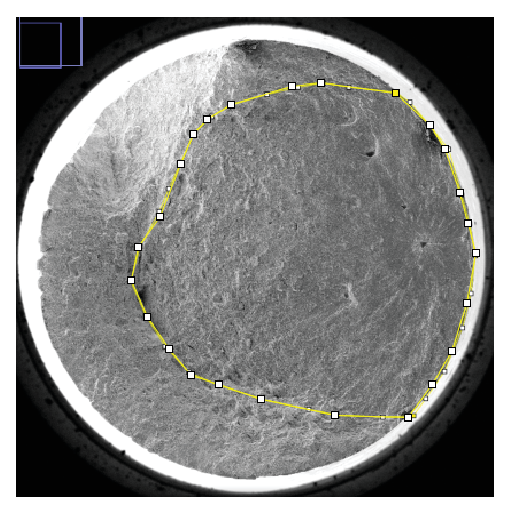
\includegraphics[width=3in]{P1MF19.eps}
  \caption{The crack in model P1MF19 marked with a yellow polygon.}
  \label{fig:P1MF19}
   \end{center}
\end{figure*}
%
The crack was marked manually.
The crack area is 11.118~mm$^2$ and the size of the ligament is $A_{\mbox{uncracked area}}=8.12$~mm$^2$.
Using eq.~(\ref{eq:sig_net}) and noting $\sigma_0=634$~MPa,
                           $\sigma_{net}=1502$~MPa.
The value found is much higher than the allowed stress $\sigma_f=1092$~MPa [how to cite Carmel confidential work??].
This finding shows the need for automatic marking of the crack.


%
%
Here continued the detail on the $\sigma_{net}$ AI model.

%%%%%%%%%%%%%%%%%%%%%%%%%%%%%%%%%%%%%%%%%%%%%%%%

Next, an example of a calculation of $K$ is presented.
The calculation is conducted for specimen P1MF19.
In order to use equation~(\ref{eq:K_I__F_I}), the crack front is approximated as an ellipse, as shown in Fig.~\ref{fig:P1MF19_elip_crack}.
%
\begin{figure*}[t!]
  \begin{center}
  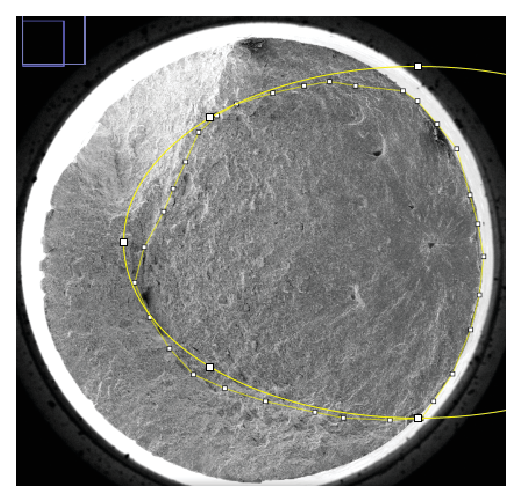
\includegraphics[width=3in]{P1MF19_elip_crack.eps}
  \caption{The crack in model P1MF19 marked with a yellow ellipse.}
  \label{fig:P1MF19_elip_crack}
   \end{center}
\end{figure*}
%
The ellipse was marked manually.
The values of $a, b$ and $D$ are 4.5~mm, 4~mm and 4.9~mm, respectively.
The range of the value $a/b$ in~\cite{shin2004experimental} is between 0 to 1.
Since here $a$ is larger than $b$, the aspect ratio between them is taken as 1.
The value of $F_I$ for $\frac{a}{b}=0, \frac{a}{D}=0.454$ and $\frac{x}{h}=0$, using eq.~(\ref{eq:F_I}), is ~1.042 (Need to be checked with the real equation. I took it from the table in~\cite{shin2004experimental}).
This is the value of $F_I$ at the middle of the crack front.
The value of $F_I$ for $\frac{a}{b}=0, \frac{a}{D}=0.454$ and $\frac{x}{h}=1$, using eq.~(\ref{eq:F_I}), is ~1.402 (kana"l).
This is the value of $F_I$ at the edges of the crack front.
Using eq.~(\ref{eq:K_I__F_I}) and noting $\sigma_0=634$~MPa, $K_I=56~\mbox{MPa}\sqrt{\mbox{m}}$ and $K_I=75\mbox{MPa}\sqrt{\mbox{m}}$ at the middle and at the edges of the crack front, respectively.
The value of the critical stress intensity factor, $K_Ic$, is $70~\mbox{MPa}\sqrt{\mbox{m}}$.
The value of $K_I$ at the middle of the crack front is much lower than the critical value.
The value of $K_I$ at the edges of the crack front is similar to the critical value.
It seems that the reason of the failure is due to the large $\sigma_{net}$ presented in Section~\ref{Subsec: Flow stress calculation model}.
The large value of $K_{Ic}$ at the edges of the crack front is unreasonable.
If the value was indeed such large, the crack should have propagated to the edges and not at the middle of the crack front.



\section{Conclusions and future work}
\label{Sec: Conclusions and future work}
\textcolor{green}{summary\\advantages of the heat map and the automatic calculation}

\section{Acknowledgments}
This work was supported by the ..


%% The Appendices part is started with the command \appendix;
%% appendix sections are then done as normal sections
%% \appendix




%\begin{thebibliography}{00}


 \bibliographystyle{elsarticle-num}
 \bibliography{bibs}




%\end{thebibliography}
\end{document}
\endinput
%%
%% End of file `elsarticle-template-num.tex'.
